\begin{adjustbox}{width=\textwidth}
	\begin{tikzpicture}[every node/.style={inner sep=0,outer sep=0}]
		% Bilder
		\node [anchor=north west] (img1) at (0,0) {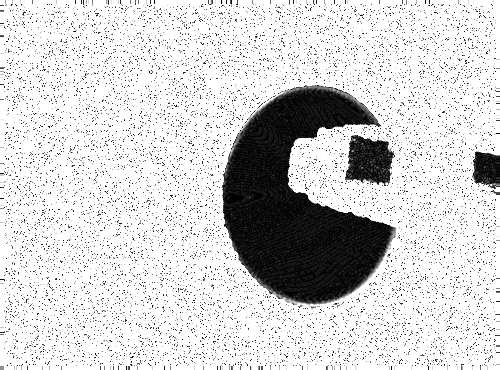
\includegraphics[width=.31\textwidth]{05_ergebnisse/ergDeflektometrischeRegistrierung/spiegelbildAuswertungDeflektometrischeRegistrierung/figures/brillenglas_1_mexican}};
		
		\node [anchor=north west] (img2) at (0.345\textwidth,0) {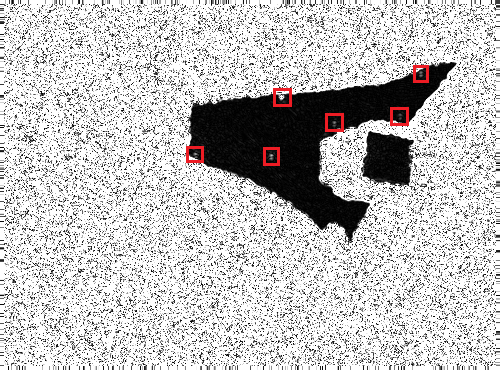
\includegraphics[width=.31\textwidth]{05_ergebnisse/ergDeflektometrischeRegistrierung/spiegelbildAuswertungDeflektometrischeRegistrierung/figures/keramikobjekt_1_mexican}};
		
		\node [anchor=north west] (img3) at (0.69\textwidth,0) {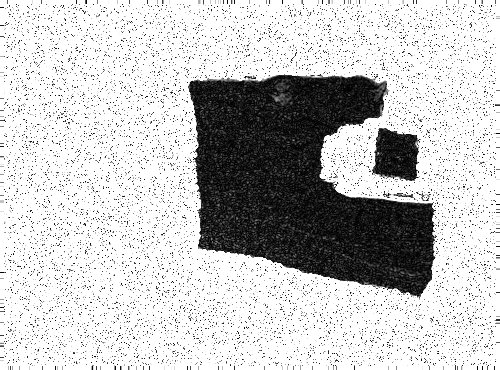
\includegraphics[width=.31\textwidth]{05_ergebnisse/ergDeflektometrischeRegistrierung/spiegelbildAuswertungDeflektometrischeRegistrierung/figures/keramikobjekt_2_mexican}};
		
		% Captions
		\node [below=0.2cm of img1] (cap1) {Brillenglas 1};
		\node [below=0.2cm of img2] (cap2) {Keramikobjekt 1};
		\node [below=0.2cm of img3] (cap3) {Keramikobjekt 2};
	\end{tikzpicture}
\end{adjustbox}
\caption[Mexican Hat-Filter angewandt auf die Bilder der deflektometrischen Registrierung der Zeilen]{Mexican Hat-Filter angewandt auf die Bilder der deflektometrischen Registrierung der Zeilen.}